\section{High Performance Computing}

\begin{frame}
    \frametitle{Computer History I}
    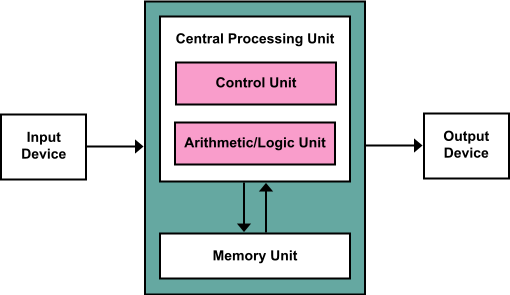
\includegraphics[width=\linewidth]{assets/von_neumann.png}

    source: \href{https://upload.wikimedia.org/wikipedia/commons/thumb/e/e5/Von_Neumann_Architecture.svg/}{Wikipedia: Von Neumann Architectures}
\end{frame}


\begin{frame}
    \frametitle{Computer History II}

    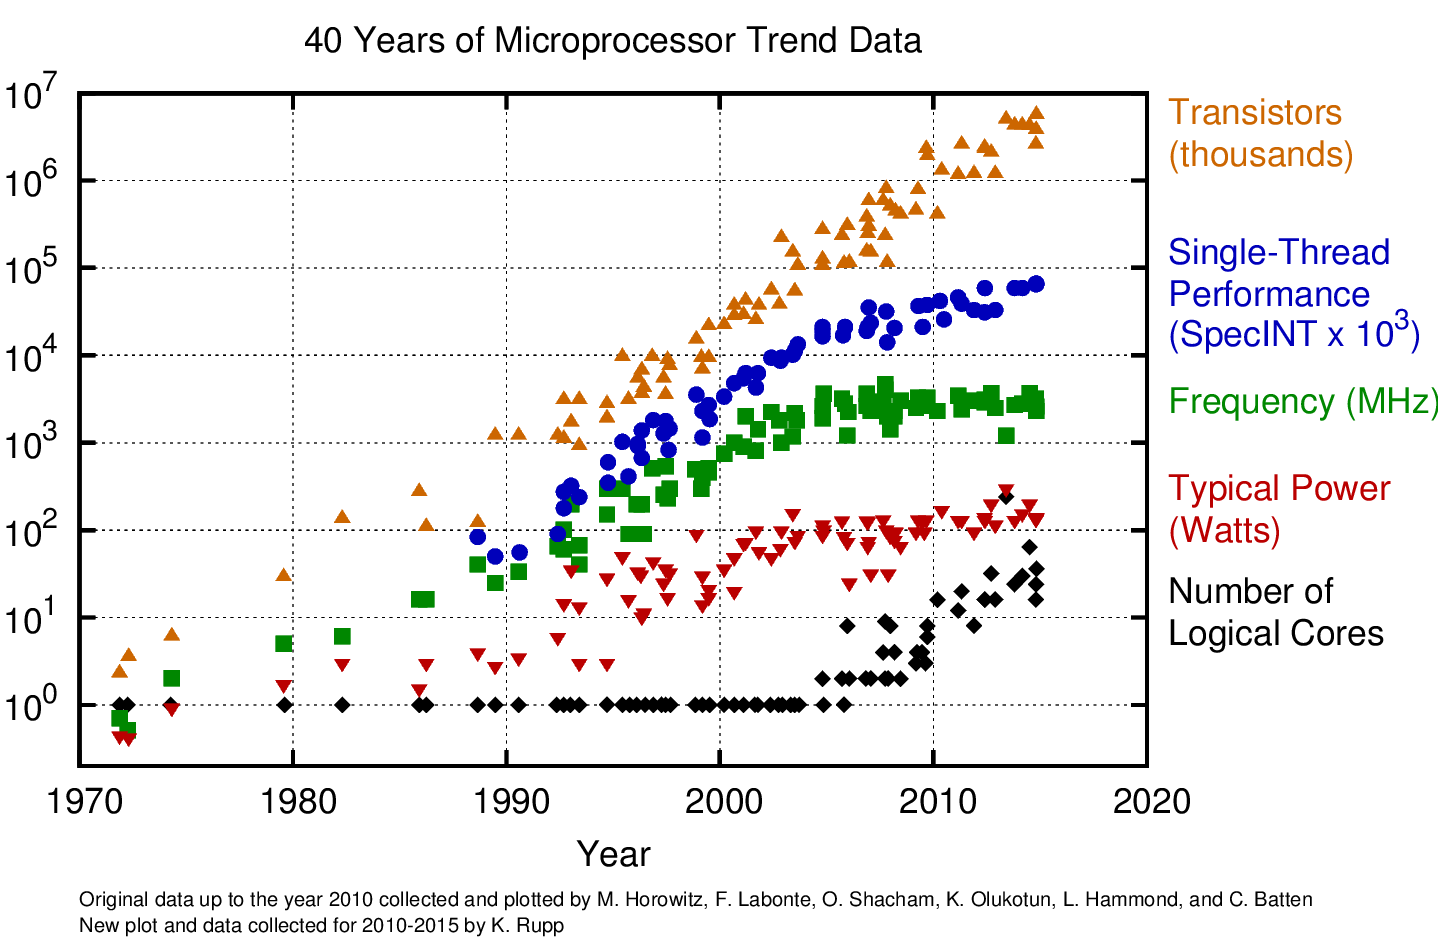
\includegraphics[width=\linewidth]{assets/dennard.png}

   source:  \href{https://arch2030.cs.washington.edu/slides/arch2030_tom_conte.pdf}{Conte, T, IEEE (2015)}
\end{frame}



\begin{frame}
    \frametitle{Computer History II}

    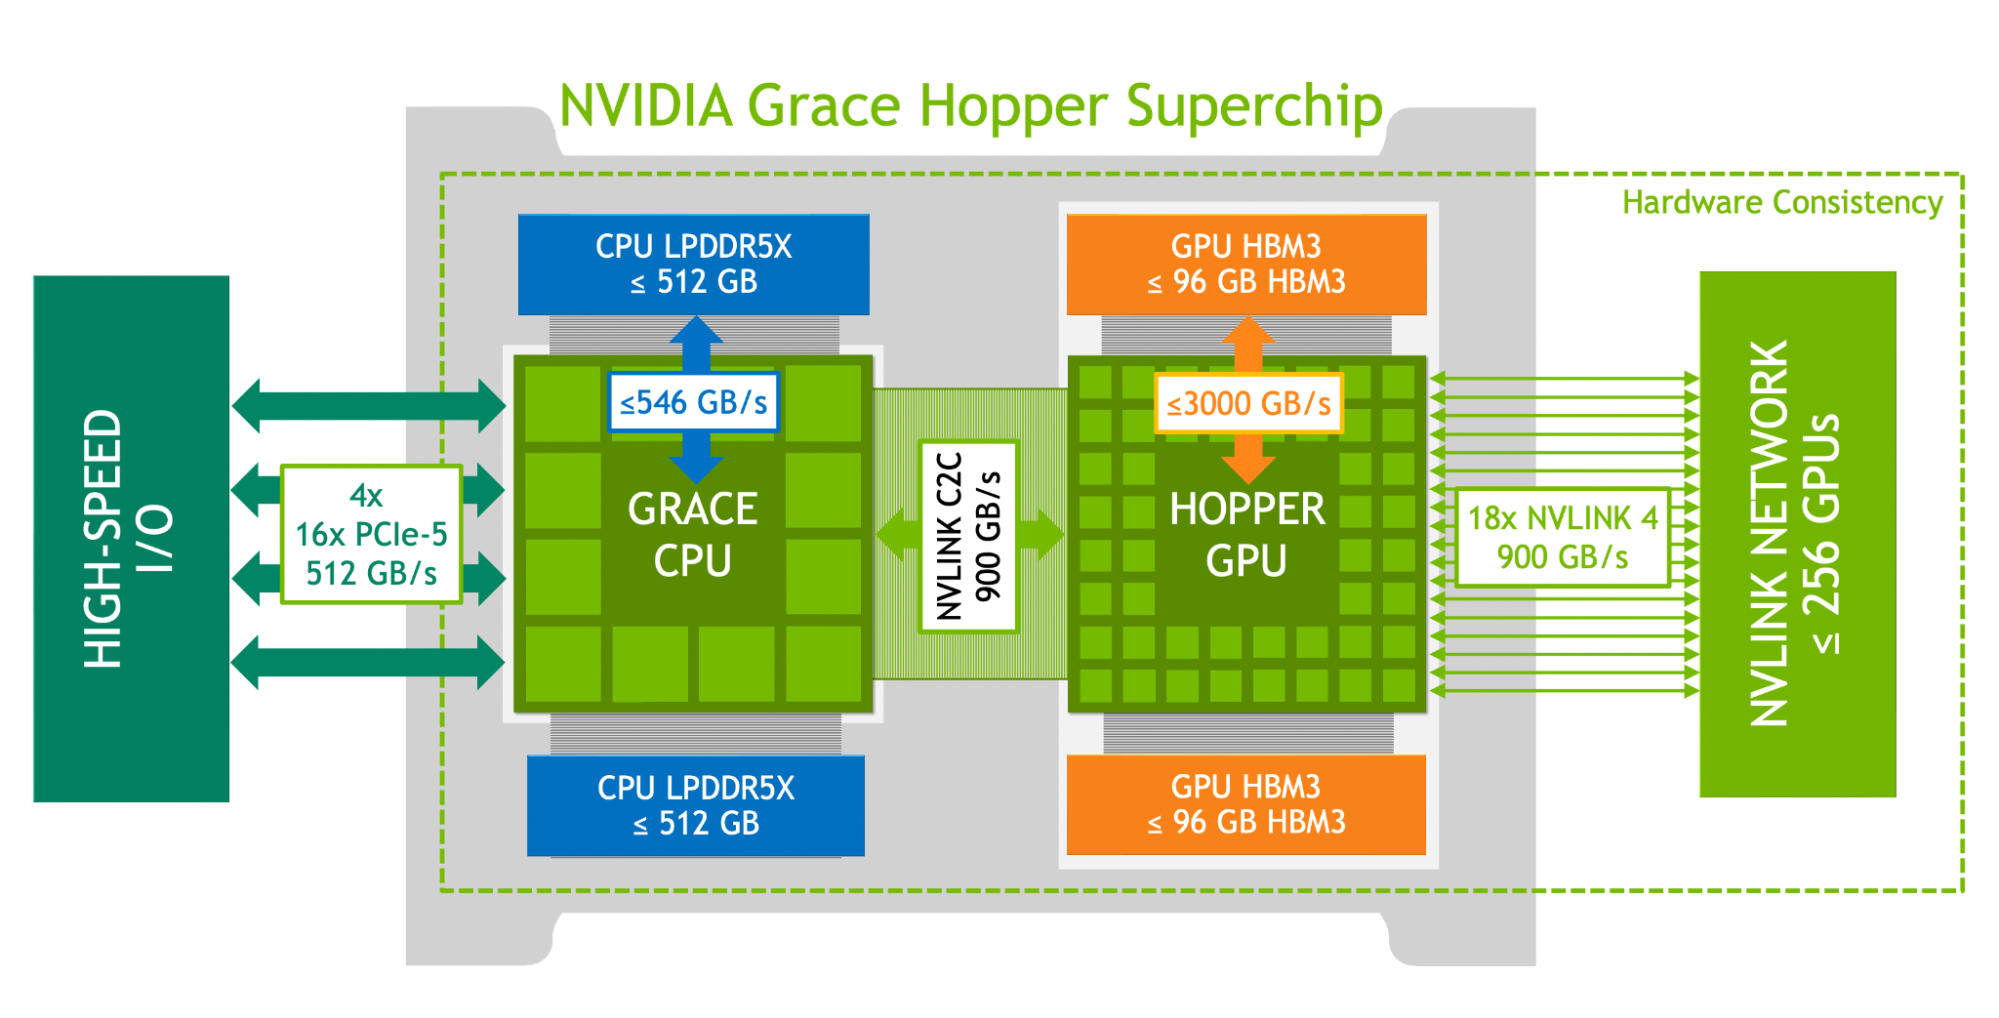
\includegraphics[width=\linewidth]{assets/grace_hopper.png}

   source:  \href{https://developer.nvidia.com/blog/nvidia-grace-hopper-superchip-architecture-in-depth/}{NVidia Corporation}
\end{frame}


\begin{frame}
    \frametitle{Computational Bottlenecks for the FMM}

    \begin{list}{-}{}

        \item \textbf{P2P} - Direct Kernel evaluations - $O(N^2)$ flops $O(N)$ memory accesses.
        \item \textbf{M2L} - Translation of the Multipole into a Local Expansion (Formulation Dependant).
    \end{list}

\end{frame}

\begin{frame}
    \frametitle{Computational Bottlenecks for the FMM II}

    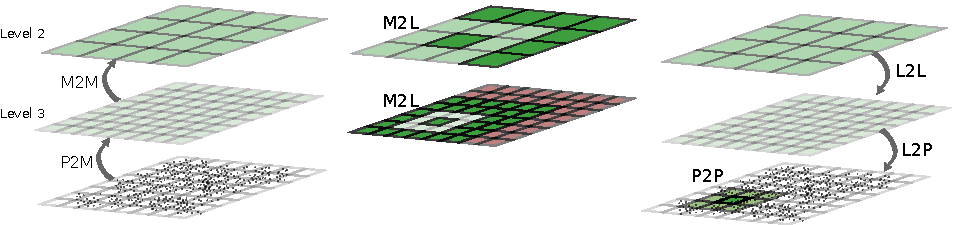
\includegraphics[width=\linewidth]{assets/algorithm.pdf}

\end{frame}


\begin{frame}
    \frametitle{The Kernel Independent FMM I}


    Consider simple test case, want to evaluate Laplace Green's function between $N$ targets $\{x_i\}_{i=1}^N$ and $N$ sources $\{y_i\}_{i=1}^N$.

    \begin{equation}
        \phi(x_i) = \sum_{j=1}^N K(x_i, y_j) q(y_j)
        \label{eq:sec:introduction:potential}
    \end{equation}

    $$ K(x, y) = \frac{1}{4\pi \||x-y\|}$$

    Want to accelerate with an FMM, to compute in $O(N)$
\end{frame}

\begin{frame}
    \frametitle{The Kernel Independent FMM II}
    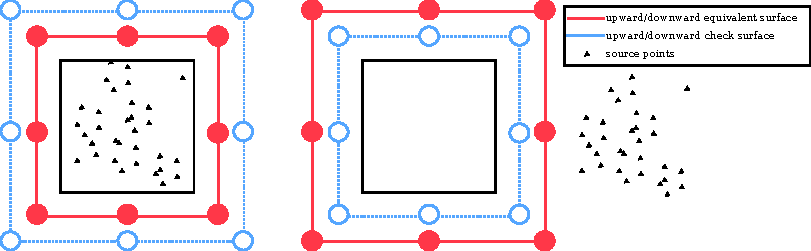
\includegraphics[width=\linewidth]{assets/p2m.pdf}
\end{frame}

\begin{frame}
    \frametitle{The Kernel Independent FMM III}
    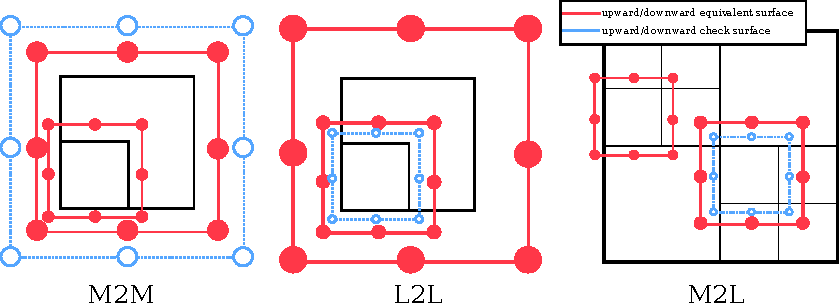
\includegraphics[width=\linewidth]{assets/translations.pdf}
\end{frame}

\begin{frame}

    Can view M2L as either a convolution (FFT) or as a dense matrix vector product (BLAS)

    \begin{equation}
        \phi^{B, d}(x) = (K \ast q)(x) = \int_{y^{B, d}} K(x-y)q^{A, u}(y)dy
        \label{eq::sec:m2l:sub:formulation:m2l_convolution}
    \end{equation}

    FFT memory throttled (notice the element-wise product), but is of only $O(N \log N)$ flops.

    \begin{equation}
        \phi(x) = \mathcal{F}^{-1}\{ \mathcal{F}\{K\}(k) \cdot \mathcal{F}\{q\}(k)  \} (x)
        \label{eq::sec:m2l:sub:formulation:m2l_convolution_matrix_2}
    \end{equation}

    BLAS is compute bound, but of $O(p^2)$ flops ...

\end{frame}

\begin{frame}
    \frametitle{Modern Implementations I}

    Modern implementations of algorithms have to reflect on advances in hardware, where we are memory bound and flops are \textit{cheap}.

    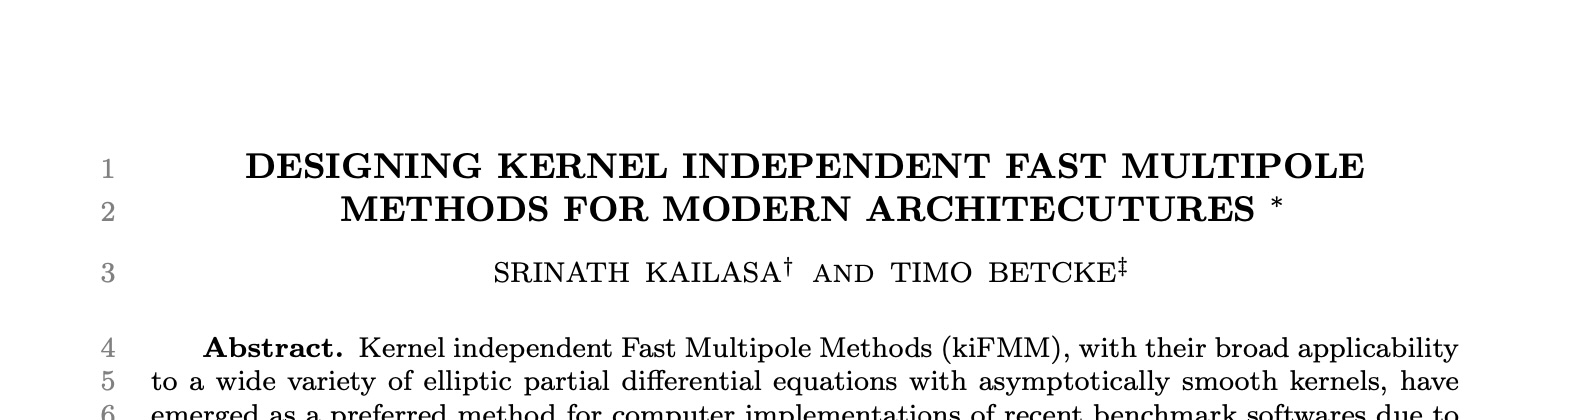
\includegraphics[width=\linewidth]{assets/upcoming.jpg}

\end{frame}


\begin{frame}
    \frametitle{Modern Implementations II }

    \begin{list}{-}{}
        \item Counterintuitively prefer a dense matrix vector product to an FFT, because of greater arithmetic intensity.
        \item Can stack together vectors which share a matrix, i.e. matrix multiplication, and get even greater data re-use.
        \item Can use numerical compression (SVD etc) to reduce size of (low-rank) matrices.
        \item Use specialised hardware and unified memory to keep the cost of GPU-CPU data exchange minimal.
    \end{list}
\end{frame}

